\documentclass[a4paper, 12pt]{article}

%---------------------------------------------------------%
%------------------ Document Preamble --------------------%
%---------------------------------------------------------%
%-------------------------------------------%
%---- First load the necessary packages ----%
%-------------------------------------------%
\usepackage{longtable}
\usepackage{booktabs}
\usepackage{graphicx}
% For including graphics (via ncludegraphics).
\usepackage{amsmath}
% Improves typographic quality of mathematical output.
\usepackage{amsfonts}
% For mathematical fonts.

% Package for no indentation and to include a line between paragraphs.
\usepackage[parfill]{parskip}

% Set the layout of the document.
\usepackage[left=2.5cm,right=2.5cm, top=1.5cm,bottom=1.5cm]{geometry}

\usepackage{amsthm} % Needed to typeset theorem environments.
\usepackage[affil-it]{authblk} % Needed for author and affiliation.
\usepackage{amsopn} % Allows the declaration of new mathematical operators.
\usepackage{amssymb} % Extended set of mathematical symbols.
\usepackage{mathrsfs} % Raph Smith's mathematical script font.
\usepackage{booktabs} % Improves the typographical quality of tables.
\usepackage{natbib} % Citations and bibliography.
\usepackage{tikz} % Extends the figure generation capabilities of LaTeX.
\usepackage{algorithm} % Necessary for including algorithmic structures.
\usepackage{float} % Allows the creation of own floating environments.
\usepackage{caption} % Allows the customisation of captions.
\usepackage{abstract} % For including abstracts in documents.
\usepackage{listings} % For the inclusion of source code.
\usepackage{color} % Used for colour commands.
\usepackage{pgfplots} %extends tikz functionality

% Automatic inclusion of hyperlinks with back references.
\usepackage[pagebackref]{hyperref}

%-------------------------------------------%

% Making a float for an algorithm.
\newfloat{algorithm}{t}{lop}
\renewcommand{\thealgorithm}{\arabic{section}.\arabic{algorithm}}

% Numbers equations by section.
\numberwithin{equation}{section}

% Add biliography
% \usepackage[style=apa,backend=biber]{biblatex}
% \usepackage[backend=biber]{biblatex}
% \addbibresource{ref.bib}
% Set biliography style.
% \bibliographystyle{apalike}

% Commands for special set of numbers.
\newcommand{\NN}{\mathbb{N}}
\newcommand{\ZZ}{\mathbb{Z}}
\newcommand{\RR}{\mathbb{R}}
\newcommand{\PP}{\mathbb{P}}
\newcommand{\EE}{\mathbb{E}}

% Commands for useful operators.
\newcommand{\di}{\text{diag}}
\newcommand{\de}{\mathrm{d}}
\newcommand{\si}{\Sigma}
\newcommand{\del}{\Delta}
\newcommand{\cov}[1]{\, {\rm cov}\left( #1 \right) }
\newcommand{\var}[1]{\, {\rm var}\left( #1 \right) }
\newcommand{\toas}{\xrightarrow{\text{a.s.}}}
\newcommand{\todis}{\xrightarrow{\text{d}}}
\newcommand{\supp}{\text{supp}}
\newcommand{\doubint}{\!\int\!\!\!\int}

% Command for text within a math sub/super-script.
\newcommand{\stext}[1]{\text{\scriptsize{#1}}}

% Command for highlighting pieces of text
\newcommand{\onote}[1]{\colorbox{orange}{#1}}

% Theorem definitions/
\newtheorem{lemma}{Lemma}[section]
\newtheorem{theorem}[lemma]{Theorem}
\newtheorem{proposition}[lemma]{Proposition}
\newtheorem{corollary}[lemma]{Corollary}

\theoremstyle{definition}
\newtheorem{definition}{Definition}[section]

\theoremstyle{remark}
\newtheorem{remark}{Remark}[section]
\newtheorem{example}[remark]{Example}

% An environment for centre aligning equations which extend past the text width.
\newenvironment{longeq}
 {\begin{displaymath}\begin{lrbox}{\overlongequation}$\displaystyle}
 {$\end{lrbox}\makebox[0pt]{\usebox{\overlongequation}}\end{displaymath}}

% Listings options.

\lstset{ %
basicstyle=\footnotesize,       % the size of the fonts that are used for the code
backgroundcolor=\color{white},  % choose the background color. You must add \usepackage{color}
showspaces=false,               % show spaces adding particular underscores
showstringspaces=false,         % underline spaces within strings
showtabs=false,                 % show tabs within strings adding particular underscores
frame=single,           % adds a frame around the code
tabsize=2,          % sets default tabsize to 2 spaces
captionpos=b,           % sets the caption-position to bottom
breaklines=true,        % sets automatic line breaking
breakatwhitespace=false,    % sets if automatic breaks should only happen at whitespace
escapeinside={\%*}{*)}          % if you want to add a comment within your code
}

%-------------------------------------------%
%------------- File Information ------------%
%-------------------------------------------%
\title{\textbf{35427962}}
\author{}
\date{}
\begin{document}
\maketitle
%-------------------------------------------%
%--------------- File Start ----------------%
%-------------------------------------------%
\begin{abstract}
The purpose of this report is to provide answers to questions 1 through 6 and to include descriptive tables and figures on which the answers are based on, and to discuss question 1 in detail using AR(1) model and provide the corresponding explanations. In conclusion, the answer to the first four questions is d, b, a, and c. The ID of 1 and 2 may suffer from high frequency attacks. The effect of the control and restraint training is not predicted to reduce the number of attacks, but it may do the opposite. However, control and restraint training may reduce the lethality of attacks.
\end{abstract}

\section*{Question I}
\subsection*{Model Fitting}
This model uses time series to quantify changes in violence over months over months. The dataset is selected and merged into groups at first, and the indicator of score given to incident is summed by month. Firstly, the graph of sequence diagram is ploted.

\begin{figure}[H]
	\centering
		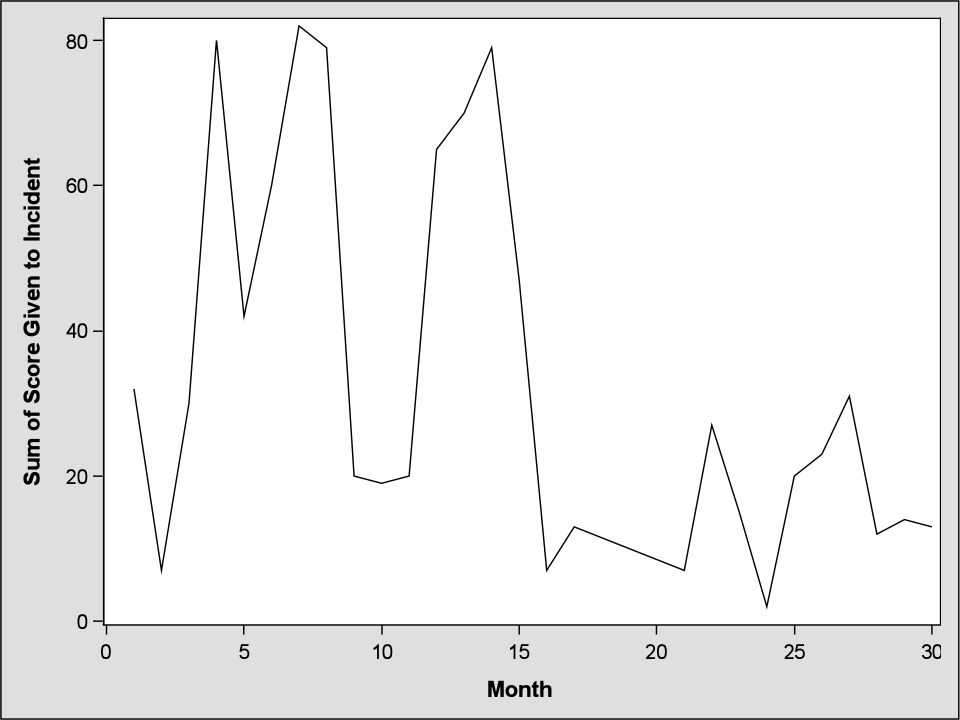
\includegraphics[scale=0.25]{Pic/Q1/1.png}
	\caption{Sequence Diagram}
	\label{f1}
\end{figure}

Based on figure of \ref{f1}, the sequence has no significant non-stationary features. White noise detection shows that there is a correlation between the sequence values, which is a non white noise sequence.

Secondly, I use three methods to solve the best parameters, namely MINIC, SCAN, and ESACF. The results of them are shown in table \ref{t1}.

\begin{table}[H]
	\centering

\begin{longtable}{rrrrrr}
\toprule
	\multicolumn{3}{c}{SCAN} &    \multicolumn{3}{c}{ESACF}\\
	\midrule
    p+d &    q &    BIC &    p+d &    q &    BIC\\
\endhead
    1 &    0 &    5.405064 &    1 &    0 &    5.405064\\
    0 &    1 &    5.60567 &    0 &    1 &    5.60567\\
     &      &      &    4 &    0 &    5.152248\\
     &      &      &    5 &    0 &    5.066185\\
\bottomrule

\caption{ARMA(p+d,q) Tentative Order Selection Tests}
\label{t1}
\end{longtable}
\end{table}

The results show that MA(5) model should be chosen. The ARIMA module of SAS is used to implement the model. After adjusting the parameters to P = 0 and Q = 5, the model results are shown in the following figure \ref{t2}.

\begin{table}[H]
\centering
\begin{longtable}{lrrrrr}
\toprule
   Parameter &    Estimate &    Standard {\newline} Error &    t~Value &    Approx {\newline} Pr > |t| &    Lag\\
\endhead
\midrule
   MU &    35.06369 &    8.46743 &    4.14 &    0.0005 &    0\\
   MA1,1 &    $-$0.69146 &    0.21930 &    $-$3.15 &    0.0048 &    1\\
   MA1,2 &    $-$0.28225 &    0.26805 &    $-$1.05 &    0.3043 &    2\\
   MA1,3 &    0.04334 &    0.28187 &    0.15 &    0.8793 &    3\\
   MA1,4 &    $-$0.02787 &    0.27443 &    $-$0.10 &    0.9201 &    4\\
   MA1,5 &    0.01157 &    0.22909 &    0.05 &    0.9602 &    5\\
\bottomrule
\caption{Conditional Least Squares Estimation of MA(5)}
\label{t2}
\end{longtable}

\begin{longtable}{lr}
\toprule
   Constant Estimate &    35.06369\\
   Variance Estimate &    552.6743\\
   Std Error Estimate &    23.50903\\
   AIC &    252.3359\\
   SBC &    260.111\\
   Number of Residuals &    27\\
\bottomrule
\caption{Model Diagnosis of MA(5)}
\label{t3}
\end{longtable}
\end{table}

According to the table \ref{t2}, we found that only two coefficients are significant. Therefore, the model should be redraft. After I calculated 121 models with P from 0 to 10 as well as Q between 0 and 10, AR(1) need to be considered since the AIC is the lowest in these models. The result of the models was given as follow.

\begin{table}[H]
\centering
\begin{longtable}{lrrrrr}
\toprule
   Parameter &    Estimate &    Standard {\newline} Error &    t~Value &    Approx {\newline} Pr > |t| &    Lag\\
\endhead
\midrule
   MU &    32.87074 &    9.17622 &    3.58 &    0.0014 &    0\\
   AR1,1 &    0.56566 &    0.16798 &    3.37 &    0.0025 &    1\\
\bottomrule
\caption{Conditional Least Squares Estimation of AR(1)}
\label{t4}
\end{longtable}
\end{table}

\begin{table}[H]
\centering
\begin{longtable}{lr}
\toprule
   Constant Estimate &    14.27693\\
   Variance Estimate &    495.1036\\
   Std Error Estimate &    22.25092\\
   AIC &    246.0734\\
   SBC &    248.6651\\
   Number of Residuals &    27\\
\bottomrule
\caption{Model Diagnosis of AR(1)}
\label{t5}
\end{longtable}
\end{table}

Comparing table \ref{t3} and \ref{t5}, we obtain the conclusion that AR(1) is much more appropriate than MA(5). In addition,, the parameters of AR(1) are significant since p-values are both less than 0.05 (Figure \ref{f2}).


\begin{figure}[H]
\centering
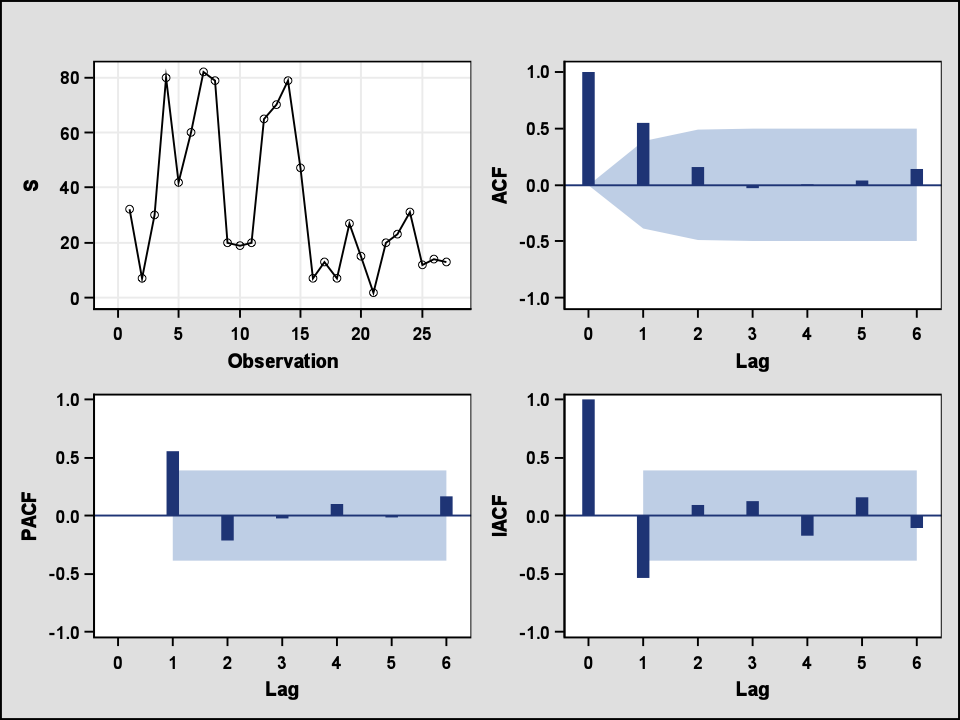
\includegraphics[scale=0.25]{Pic/Q1/2.png}
\caption{Trend and Correlation Analysis for Sum of Score Given to Incident}
\label{f2}
\end{figure}

Thirdly, according to the autocorrelation coefficient in figure \ref{f2}, except for the autocorrelation coefficients of the first order delay being instead of are in the range of twice standard deviation, the autocorrelation coefficients of other orders fluctuate in the range of twice standard deviation. Based on this feature, we can judge that the sequence has short-term correlation, and further confirm that the sequence is stable. Furthermore, the process of the partial autocorrelation coefficient decaying to zero is further investigated. Except the first order partial autocorrelation coefficient being instead of is in the range of double standard deviation, the other order partial autocorrelation coefficients are in the range of double standard deviation, which is a typical characteristic of the first-order truncated partial autocorrelation coefficient.

Finally, according to the table \ref{t4}, the fomula of AR(1) can be demonstrated as follow.

\begin{equation}
x_{t} = 32.87074 + 0.56566\times x_{t-1} + \epsilon_{t}, Var(\epsilon_{t}) = 495.1036
\label{e1}
\end{equation}

where $x_{t}$ is sum of score given to incident by month t.

\begin{figure}[H]
\centering
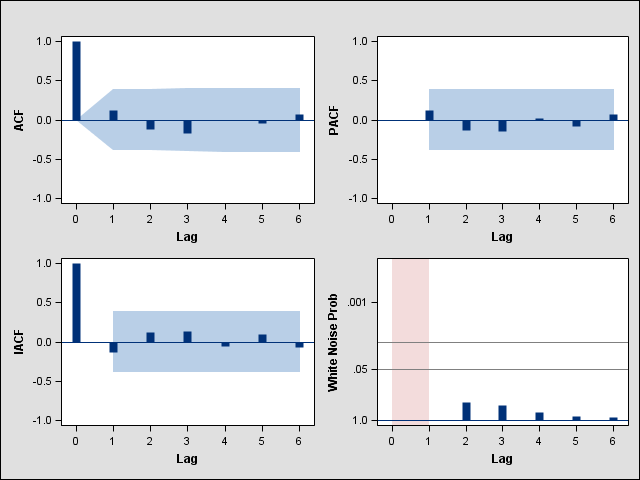
\includegraphics[scale=0.5]{Pic/Q1/3.png}
\caption{Residual Correlation Diagnostics for Sum of Score Given to Incident}
\label{f3}
\end{figure}

\begin{figure}[H]
\centering
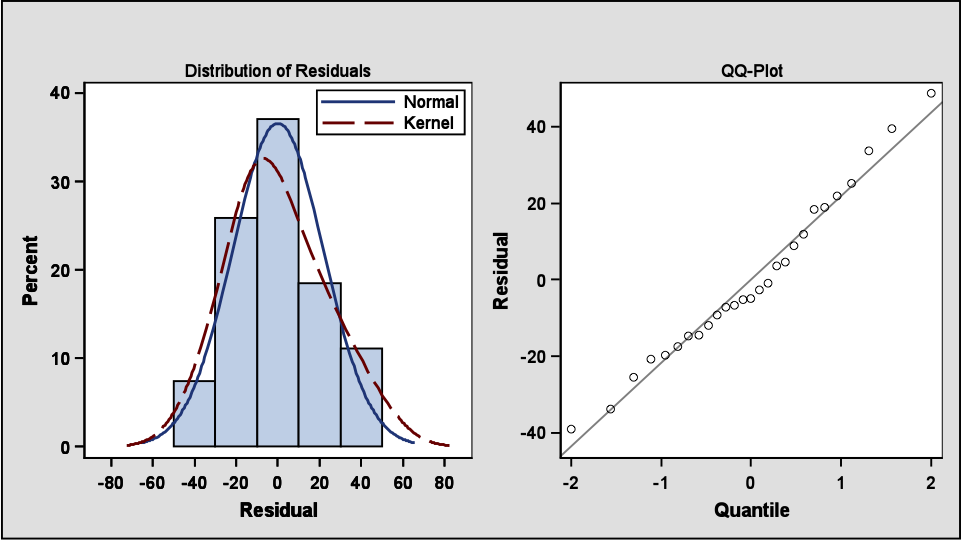
\includegraphics[scale=0.25]{Pic/Q1/4.png}
\caption{Residual Normality Diagnostics for Sum of Score Given to Incident}
\label{f4}
\end{figure}

These two figures (\ref{f2}, \ref{f3}) show that the effect of the model is good. The residual error of the model is in line with normal distribution from the chart of QQ plot.

\subsection*{Hypothesis testing}

The significance test of model \ref{e1} is white noise test of residual sequence. Therefore, the null hypothesis and alternative hypothesis are:

$$H_{0}: \rho_{1} = 0, \forall m \ge 1$$
$$H_{1}: \exists \rho_{k}\neq 0, \forall m \ge 1, k\le m$$

The test statistic is LB (Ljung-Box):

$$LB = n(n + 2) \sum_{k=1}^{m}(\frac{\hat{\rho_{k}}^{2}}{n-k})\sim \chi^{2}(m), \forall m > 0$$

If the null hypothesis is rejected, it means that there are still some relevant information in the residual sequence, and the fitting model is not significant. If the original hypothesis cannot be rejected, the fitting model is considered significant. The result is given as table \ref{tlb}.

\begin{table}[H]
\begin{longtable}{rrrrrrrrrr}
\toprule
   To Lag &    Chi-Square &    DF &    Pr > ChiSq &    \multicolumn{6}{c}{Autocorrelations}\\
  \midrule
\endhead
   6 &    10.73 &    6 &    0.0969 &    0.551 &    0.155 &    $-$0.032 &    0.002 &    0.036 &    0.142\\
\bottomrule
\caption{Autocorrelation Check for White Noise}
\label{tlb}
\end{longtable}
\end{table}

It can be seen from the results that p-value is 0.0969, which is greater than 0.05. Therefore, we cannot reject the null hypothesis. This is a good proof that the data is a very stable white noise sequence. In conclusion, this model proves the fact that the trends in violence is non-monotonic over time. The option D may be the correct answer.


\section*{Question II}

\begin{figure}[H]
\centering
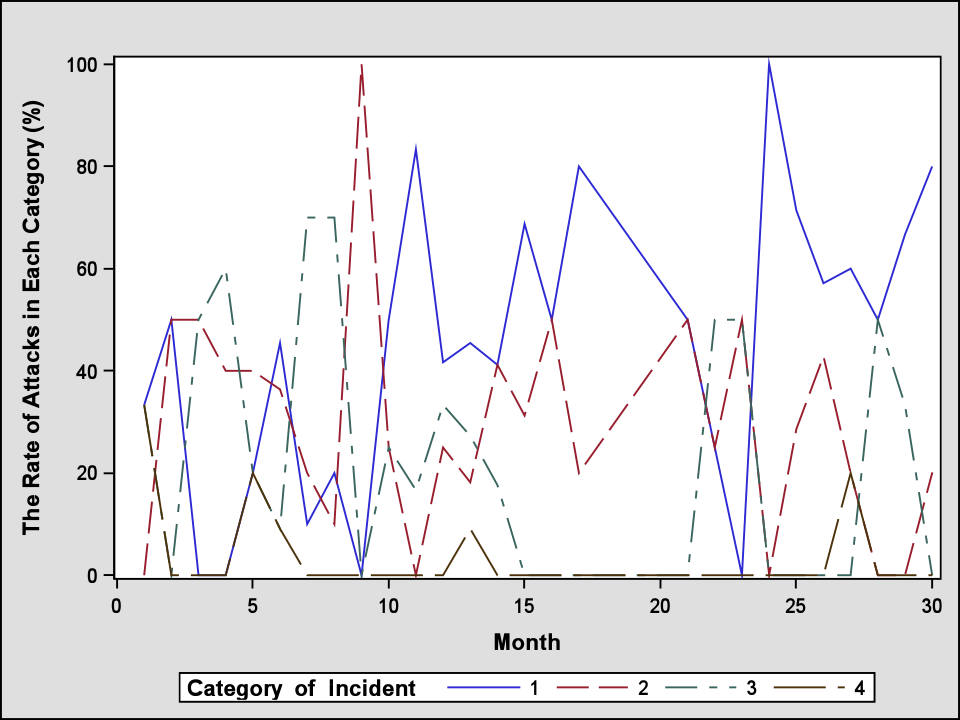
\includegraphics[scale=0.25]{Pic/Q2/1.png}
\caption{The Rate of Attacks in Each Category}
\label{f5}
\end{figure}

At the outset, we can see that it is not the same throughout the 30-month period by the figure \ref{f5} above.

\begin{figure}[htbp]
\centering
\begin{minipage}[t]{0.48\textwidth}
\centering
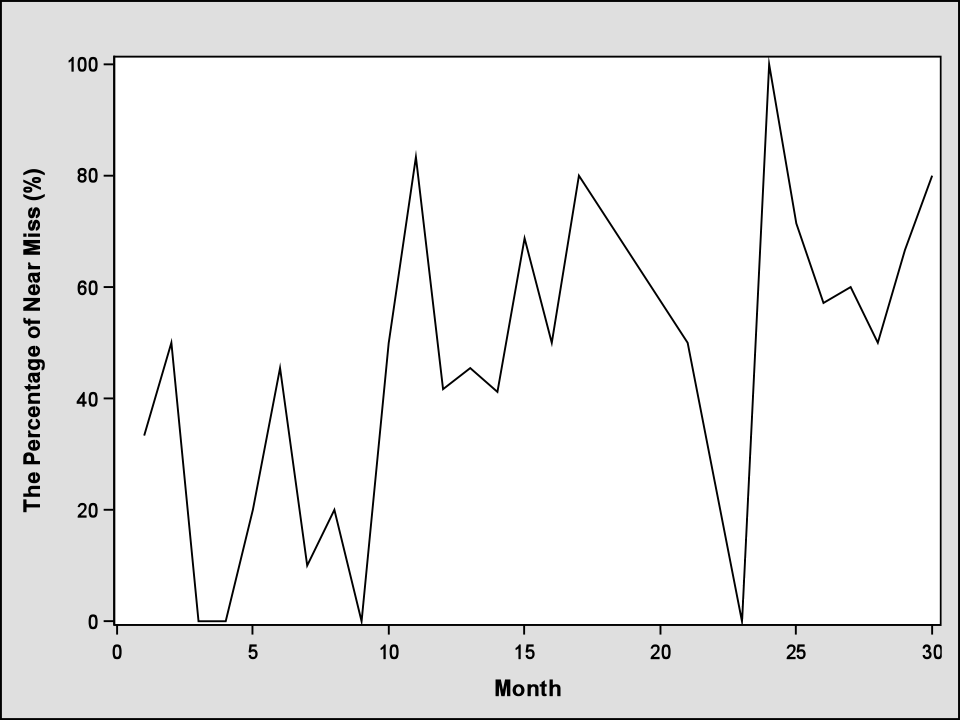
\includegraphics[width=6cm]{Pic/Q2/2.png}
\caption{The Percentage of Near Miss}
\label{f6}
\end{minipage}
\begin{minipage}[t]{0.48\textwidth}
\centering
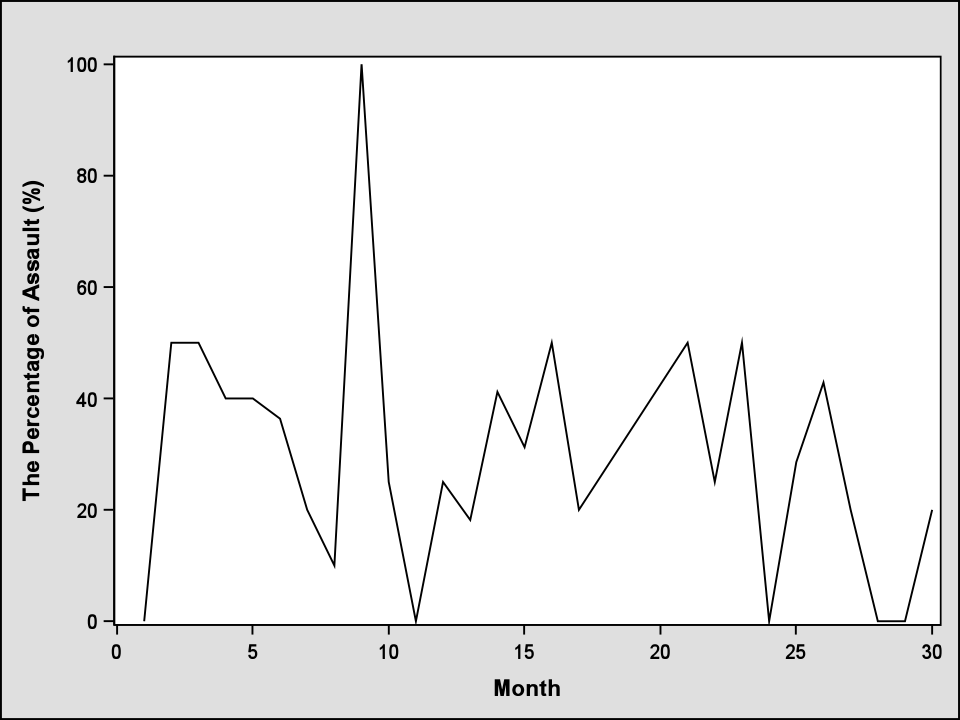
\includegraphics[width=6cm]{Pic/Q2/3.png}
\caption{The Percentage of Assault}
\label{f7}
\end{minipage}
\end{figure}

Moreover, these two figures (\ref{f6}, \ref{f7}) show that is not always
proportional to the number of attacks each month.

\begin{figure}[H]
\centering
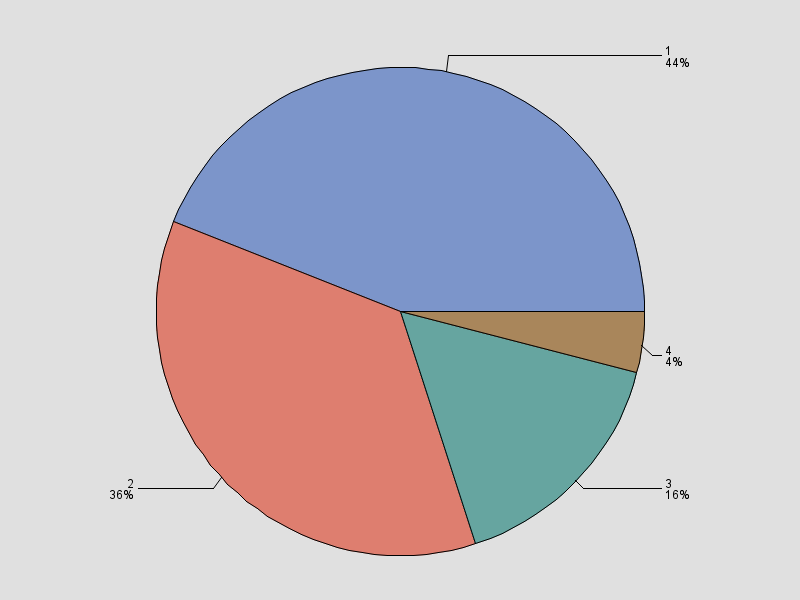
\includegraphics[scale=0.5]{Pic/Q2/4.png}
\caption{The Rate of Attacks in Each Category for the Second Half
of the 30 Months}
\label{f8}
\end{figure}
Finally, figure (\ref{f8}) shows that there was a higher proportion of less threatening incidents in the second half
of the 30 months. In conclusion, these figures demonstrate the fact that less threatening incidents accounts a higher proportion. The option B may be the correct answer.


\section*{Question III}

I used ANOVA model to compare the influence of gender on violence at different levels. Table \ref{t9} shows the model output.

\begin{table}[H]
\centering
\begin{longtable}{lrrrrr}
\toprule
   Source &    DF &    Sum of Squares &    Mean Square &    F Value &    Pr~>~F\\
\endhead
\midrule
   Model &    6 &    2806.376471 &    467.729412 &    Infty &    <.0001\\
   Error &    163 &    0.000000 &    0.000000 &      &     \\
   Corrected Total &    169 &    2806.376471 &      &      &     \\
\bottomrule
\end{longtable}

\begin{longtable}{rrrr}
\toprule
   R-Square &    Coeff Var &    Root MSE &    Score given to incident~Mean\\
\endhead
\midrule
   1.000000 &    0 &    0 &    5.388235\\
\bottomrule
\end{longtable}

\begin{longtable}{lrrrrr}
\toprule
   Source &    DF &    Anova SS &    Mean Square &    F Value &    Pr~>~F\\
\endhead
\midrule
   Sex*Category &    6 &    2806.376471 &    467.729412 &    Infty &    <.0001\\
\bottomrule
\end{longtable}

\caption{ANOVA of the Interaction between Sex of Perpetrator and Category of Incident}
\label{t6}
\end{table}

\begin{table}[H]
\centering
\begin{longtable}{llrrr}
\toprule
   Level of {\newline} Sex of Perpetrator &    Level of {\newline} Category of Incident &    N &    \multicolumn{2}{c}{Score Given to Incident}\\

   ~ &    ~ &    ~ &    Mean &    Std Dev\\
\endhead
\midrule
   F &    1 &    37 &    2.0000000 &    0\\
   F &    2 &    31 &    5.0000000 &    0\\
   F &    3 &    30 &    10.0000000 &    0\\
   M &    1 &    36 &    2.0000000 &    0\\
   M &    2 &    19 &    5.0000000 &    0\\
   M &    3 &    12 &    10.0000000 &    0\\
   M &    4 &    5 &    20.0000000 &    0\\
\bottomrule
\caption{Mean of the Interaction between Sex of Perpetrator and Category of Incident}
\label{t7}

\end{longtable}
\end{table}

\begin{figure}[H]
\centering
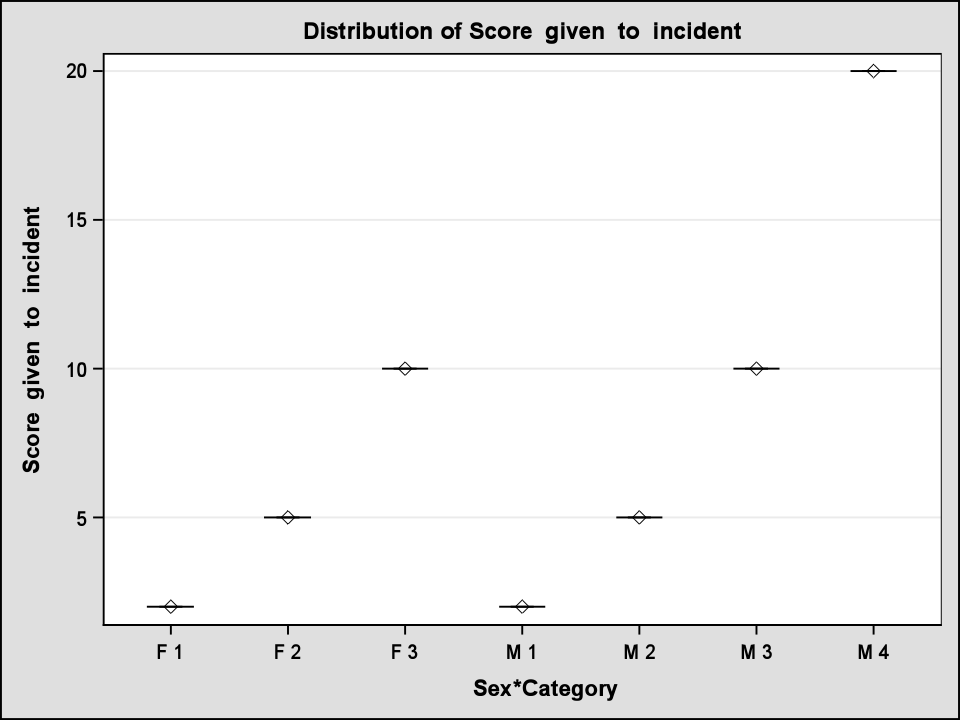
\includegraphics[scale=0.25]{Pic/Q3/3.png}
\caption{ANOVA of the Interaction between Sex of Perpetrator and Category of Incident}
\label{f9}
\end{figure}

According to the table \ref{t6}, we can see p-value is less than 0.0001. Therefore, it is sure that gender has an impact on different levels of violence. The results showed that men were more likely to cause fatal attacks. The option A may be the correct answer.




\section*{Question IV}

\begin{figure}[H]
\centering
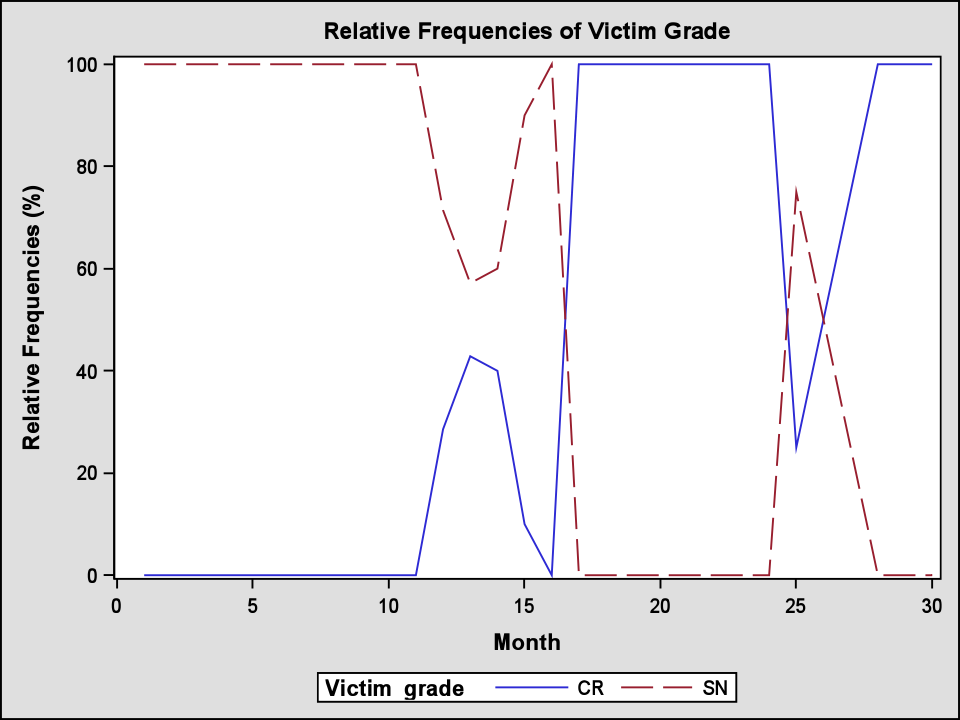
\includegraphics[scale=0.25]{Pic/Q4/1.png}
\caption{Relative Frequencies of Victim Grade}
\label{f10}
\end{figure}

As can be seen from figure \ref{f10}, the relative frequency of the victim's grade changes over time. As a result, the option C may be chosen.

\section*{Question V}

\begin{figure}[H]
\centering
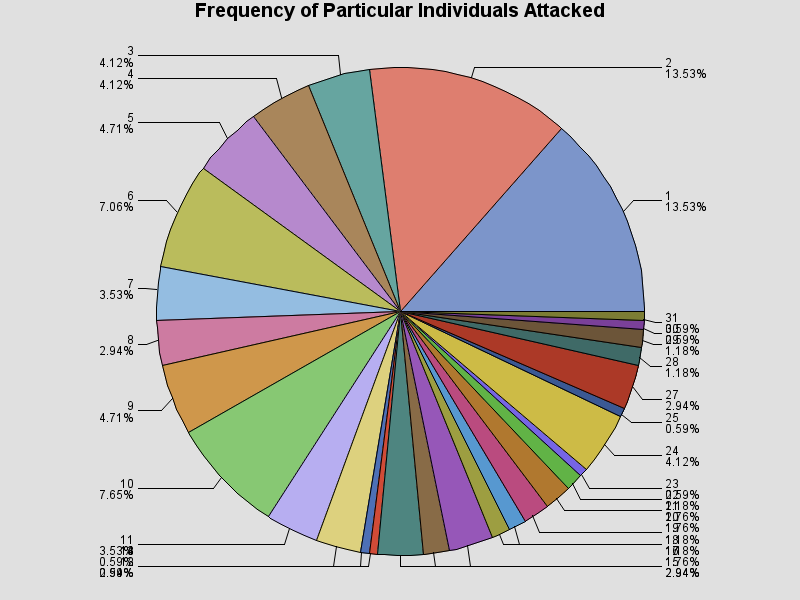
\includegraphics[scale=0.5]{Pic/Q5/1.png}
\caption{Freauency of Particular Individuals Attacked}
\label{f11}
\end{figure}

The ID of 1 and 2 received the high frequency of attacks from figure \ref{f11}. Therefore, I would like to select option A.


\section*{Question VI}

\begin{table}[H]
\centering
\begin{longtable}{lrrrrrrr}
\toprule
   Parameter &    DF &    Estimate &    Std. &    \multicolumn{2}{c}{Wald 95\% Confidence Limits} &    Wald $\chi^{2}$ &    Pr~>~$\chi^{2}$\\
\endhead
\midrule
   Intercept &    1 &    1.1835 &    0.2542 &    0.6853 &    1.6816 &    21.68 &    <.0001\\
   CRStaff &    1 &    0.0257 &    0.0169 &    $-$0.0074 &    0.0588 &    2.32 &    0.1280\\
   Scale &    0 &    1.0000 &    0.0000 &    1.0000 &    1.0000 &      &     \\
\bottomrule
\caption{Analysis of Maximum Likelihood Parameter Estimates}
\label{t8}
\end{longtable}

\begin{longtable}{lrrr}
\toprule
   Criterion &    DF &    Value &    Value/DF\\
\endhead
\midrule
   Deviance &    33 &    236.4986 &    7.1666\\
   Scaled Deviance &    33 &    236.4986 &    7.1666\\
   Pearson Chi-Square &    33 &    363.4218 &    11.0128\\
   Scaled Pearson X2 &    33 &    363.4218 &    11.0128\\
   Log Likelihood &      &    90.4709 &     \\
   Full Log Likelihood &      &    $-$167.2711 &     \\
   AIC (smaller is better) &      &    338.5421 &     \\
   AICC (smaller is better) &      &    338.9171 &     \\
   BIC (smaller is better) &      &    341.6528 &     \\
\bottomrule
\caption{Criteria for Assessing Goodness of Fit}
\label{t9}
\end{longtable}
\end{table}

I use Poisson's generalized linear model to fit the number of attacks and the number of staffs who are received the control and restraint training. The results are shown in the table (\ref{t8}, \ref{t9}). It can be clearly seen that the more people are trained, the more times they attack.

\begin{table}[H]
\centering
\begin{longtable}{lrrr}
\toprule
   Test &    Chi-Square &    DF &    Pr~>~ChiSq\\
\endhead
\midrule
   Likelihood Ratio &    25.3116 &    1 &    <.0001\\
   Score &    23.9340 &    1 &    <.0001\\
   Wald &    23.0210 &    1 &    <.0001\\
\bottomrule
\caption{Testing Global Null Hypothesis: BETA=0}
\label{t10}
\end{longtable}

\begin{longtable}{llrrrrr}
\toprule
   Parameter &    ~ &    DF &    Estimate &    Standard {\newline} Error &    Wald {\newline} Chi-Square &    Pr~>~ChiSq\\
\endhead
\midrule
   Intercept &    2 &    1 &    $-$2.2009 &    0.4307 &    26.1110 &    <.0001\\
   Intercept &    5 &    1 &    $-$0.7888 &    0.3972 &    3.9441 &    0.0470\\
   Intercept &    10 &    1 &    1.8759 &    0.5565 &    11.3625 &    0.0007\\
   CRStaff &      &    1 &    0.1560 &    0.0325 &    23.0210 &    <.0001\\
\bottomrule
\caption{Analysis of Maximum Likelihood Estimates}
\label{t11}
\end{longtable}
\end{table}

\begin{figure}[H]
\centering
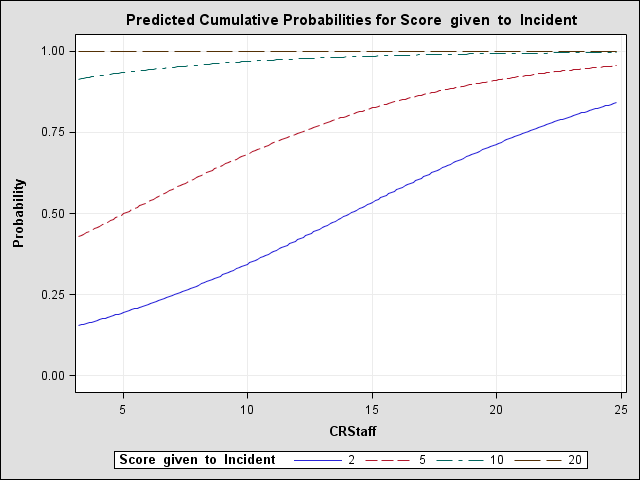
\includegraphics[scale=0.5]{Pic/Q6/1.png}
\caption{Predicted Cumulative Probabilities for Score Given to Incident}
\label{f12}
\end{figure}

The logistic model is used to fit the relationship between the severity of attack and the number of trained employees. According to the figure \ref{f12}, the more people are trained, the more obvious the probability of low-level injuries. This means that increasing the number of trainees will reduce the occurrence of high-level attacks, but not the number of attacks.


\clearpage

\section*{Appendix}

\subsection*{SAS Code}

\lstset{language=SAS}
\begin{lstlisting}
/*Load Data*/
DATA CW.violence;
LIBNAME CW 'D:\RemoteFiles\CW\Data';
INFILE 'D:\RemoteFiles\CW\Data\violence.dat';
INPUT Incident_number Month Category_of_incident Score_given_to_incident ID_of_perpetrator Sex_of_perpetrator $ Each_attack_of_perpetrator Last_attack_of_perpetrator ID_of_victim Sex_of_victim $ Each_attack_on_victim Last_attack_on_victim Victim_grade $ CRStaff;
PROC PRINT DATA=CW.violence;
RUN;

/*Question 1*/
DATA W1;
SET CW.violence (KEEP = Month Score_given_to_incident);
PROC SQL;
	CREATE TABLE CW.Q1 AS
	SELECT Month, SUM(Score_given_to_incident) as S
	FROM W1
	GROUP BY Month;
QUIT;
PROC SGPLOT;
	SERIES X = Month Y = S;
	YAXIS LABEL="Sum of Score Given to Incident";
RUN;
PROC ARIMA;
	IDENTIFY VAR=S MINIC SCAN ESACF;
RUN;
PROC ARIMA;
	IDENTIFY VAR=S;
	ESTIMATE P=0 Q=5 PLOT;
RUN;
PROC ARIMA;
	IDENTIFY VAR=S;
	ESTIMATE P=1 Q=0 PLOT;
RUN;
QUIT;

/*Question 2*/
DATA W2;
SET CW.violence (KEEP = Month Category_of_incident);
PROC SQL;
	CREATE TABLE CW.Q2 AS
	SELECT Month, Category_of_incident, COUNT(Month) AS C
	FROM W2
	GROUP BY Month, Category_of_incident
	ORDER BY Month, Category_of_incident;
QUIT;
PROC SQL;
	CREATE TABLE CW.Q2_1 AS
	SELECT Month, Category_of_incident, C, SUM(C) AS Month_C, C / SUM(C) * 100 AS Category_RATE
	FROM CW.Q2
	GROUP BY Month
	ORDER BY Month, Category_of_incident;
QUIT;
DATA CW.Q2_0;
INPUT Month Category_of_incident C Month_C Category_RATE;
CARDS;
1 2 0 0 0.0
\end{lstlisting}
\begin{lstlisting}
2 3 0 0 0.0
2 4 0 0 0.0
3 1 0 0 0.0
3 4 0 0 0.0
4 1 0 0 0.0
4 4 0 0 0.0
7 4 0 0 0.0
8 4 0 0 0.0
9 1 0 0 0.0
9 3 0 0 0.0
9 4 0 0 0.0
10 4 0 0 0.0
11 2 0 0 0.0
11 4 0 0 0.0
12 4 0 0 0.0
14 4 0 0 0.0
15 3 0 0 0.0
15 4 0 0 0.0
16 3 0 0 0.0
16 4 0 0 0.0
17 3 0 0 0.0
17 4 0 0 0.0
21 3 0 0 0.0
21 4 0 0 0.0
22 4 0 0 0.0
23 1 0 0 0.0
23 4 0 0 0.0
24 2 0 0 0.0
24 3 0 0 0.0
24 4 0 0 0.0
25 3 0 0 0.0
25 4 0 0 0.0
26 3 0 0 0.0
26 4 0 0 0.0
27 3 0 0 0.0
28 2 0 0 0.0
28 4 0 0 0.0
29 2 0 0 0.0
29 4 0 0 0.0
30 3 0 0 0.0
30 4 0 0 0.0
;
RUN;

/*Optian a*/
DATA CW.Q2_2;
	SET CW.Q2_0 CW.Q2_1;
RUN;
PROC SORT DATA=CW.Q2_2;
	BY MONTH Category_of_incident;
RUN;
PROC SGPLOT DATA=CW.Q2_2;
	SERIES X = Month Y = Category_RATE / GROUP = Category_of_incident;
	YAXIS LABEL="The Rate of Attacks in Each Category (%)";
	TITLE '';
RUN;
DATA CW.Q2_2_near_miss;
	SET CW.Q2_2 (KEEP = Month Category_of_incident Category_RATE);
	WHERE  Category_of_incident = 1;
RUN;
PROC SGPLOT DATA=CW.Q2_2_near_miss;
	SERIES X = Month Y = Category_RATE;
\end{lstlisting}
\begin{lstlisting}
	TITLE '';
	YAXIS LABEL="The Percentage of Near Miss (%)";
RUN;

DATA CW.Q2_2_assault;
	SET CW.Q2_2 (KEEP = Month Category_of_incident Category_RATE);
	WHERE  Category_of_incident = 2;
RUN;
PROC SGPLOT DATA=CW.Q2_2_assault;
	SERIES X = Month Y = Category_RATE;
	TITLE '';
	YAXIS LABEL='The Percentage of Assault (%)';
RUN;
DATA W2_1;
	SET CW.violence (KEEP = Month Category_of_incident);
PROC SQL;
	CREATE TABLE W2_Total AS
	SELECT Month, COUNT(Month) AS C
	FROM W2_1
	GROUP BY Month
	ORDER BY Month;
QUIT;
PROC SQL;
	CREATE TABLE W2_Assault AS
	SELECT Month, COUNT(Month) AS A
	FROM W2_1
	WHERE Category_of_incident = 2
	GROUP BY Month
	ORDER BY Month;
QUIT;
DATA Q2_Merged;
	MERGE W2_Total W2_Assault;
	BY Month;
	RETAIN Assault;
	IF A = . THEN Assault = 0;
	ELSE Assault = A;
PROC CORR DATA=Q2_Merged ;
	VAR C Assault;
RUN;

/*Optian (b)*/
DATA CW.Q2_3;
	SET CW.Q2_1;
	WHERE Month > 15;
	Category = PUT(Category_of_incident, 2.);
	DROP Category_of_incident;
PROC GCHART DATA=CW.Q2_3;
	PIE Category /
	VALUE=NONE
	PERCENT=ARROW
	SLICE=ARROW
	NOHEADING;
	TITLE '';
RUN;
QUIT;

/*Question 3*/
DATA CW.Q3;
	SET CW.violence (KEEP = Category_of_incident Score_given_to_incident Sex_of_perpetrator);
PROC ANOVA DATA=CW.Q3;
	CLASS Sex_of_perpetrator Category_of_incident;
\end{lstlisting}
\begin{lstlisting}
	MODEL Score_given_to_incident=Sex_of_perpetrator Category_of_incident Sex_of_perpetrator*Category_of_incident;
	MEANS Sex_of_perpetrator Category_of_incident Sex_of_perpetrator*Category_of_incident/DUNCAN;
RUN;
PROC SQL;
	CREATE TABLE CW.Q3_1 AS
	SELECT Sex_of_perpetrator, Category_of_incident, SUM(Each_attack_of_perpetrator) AS Each_SUM
	FROM CW.violence
	GROUP BY Category_of_incident, Sex_of_perpetrator
	ORDER BY Category_of_incident, Sex_of_perpetrator;
QUIT;
PROC GCHART DATA=CW.Q3_1;
	VBAR Sex_of_perpetrator /SUMVAR=Each_SUM GROUP=Category_of_incident;
	TITLE 'Score Given to Incident by Sex';
RUN;

/*Question 4*/
DATA CW.Q4;
	SET CW.violence (KEEP=Month Victim_grade);
	WHERE Victim_grade = "SN" OR Victim_grade = "CR";
PROC FREQ DATA=CW.Q4;
	TABLES Month * Victim_grade /OUT=W4_FREQ OUTPERCENT;
RUN;
PROC PRINT DATA=W4_FREQ;
RUN;
DATA W4_FREQ_1;
	SET W4_FREQ (KEEP=Month Victim_grade PCT_ROW);
	PCT_ROW = PCT_ROW;
DATA W4_FREQ_0;
INPUT Month Victim_grade $ PCT_ROW;
CARDS;
1 CR 0.00000
2 CR 0.00000
3 CR 0.00000
4 CR 0.00000
5 CR 0.00000
6 CR 0.00000
7 CR 0.00000
8 CR 0.00000
9 CR 0.00000
11 CR 0.00000
16 CR 0.00000
17 SN 0.00000
24 SN 0.00000
28 SN 0.00000
29 SN 0.00000
30 SN 0.00000
;
DATA CW.Q4_FREQ;
	SET W4_FREQ_1 W4_FREQ_0;
PROC SORT DATA=CW.Q4_FREQ;
	BY Month Victim_grade;
RUN;
PROC SGPLOT DATA=CW.Q4_FREQ;
	SERIES X = Month Y = PCT_ROW/GROUP=Victim_grade;
	TITLE 'Relative Frequencies of Victim Grade';
	YAXIS LABEL='Relative Frequencies';
RUN;

/*Question 5*/
\end{lstlisting}
\begin{lstlisting}
DATA CW.Q5;
	SET CW.violence (KEEP=ID_of_victim);
	ID = PUT(ID_of_victim, 2.);
	DROP ID_of_victim;
RUN;
PROC FREQ DATA=CW.Q5;
	TABLES ID/OUT=CW.Q5_FREQ;
RUN;
PROC GCHART DATA=CW.Q5;
	PIE ID /
	VALUE=NONE
	PERCENT=ARROW
	SLICE=ARROW
	NOHEADING
	OTHER=0;
	TITLE 'Frequency of Particular Individuals Attacked';
RUN;
QUIT;

/*Question 6*/
/*number*/
DATA CW.Q6_Number;
	SET CW.violence (KEEP=Each_attack_of_perpetrator Last_attack_of_perpetrator CRStaff);
	WHERE Last_attack_of_perpetrator = 1;
PROC GENMOD DATA=CW.Q6_Number PLOTS=ALL;
	MODEL Each_attack_of_perpetrator = CRStaff / DIST=POSSION LINK = LOG;
	OUTPUT OUT=bclassg_Number p=pred_Number;
RUN;
/*severity of the attacks*/
DATA CW.Q6_Severity;
	SET CW.violence (KEEP=Category_of_incident Score_given_to_incident Each_attack_of_perpetrator CRStaff);
PROC LOGISTIC PLOTS=ALL;
	MODEL Score_given_to_incident=CRStaff;
	OUTPUT OUT=bclassg_Severity p=pred_Severity;
RUN;
QUIT;
\end{lstlisting}


\end{document}
